\subsection{Solve Problem}
\begin{frame}{Solve Problem}
\begin{figure}[H]
	\centering
		\includegraphics[width=1.00\textwidth, clip=true, trim=4cm 10.5cm 8cm 8cm]{input/alex_before.png}
	\label{fig:alex_before}
\end{figure}

\begin{figure}[H]
	\centering
		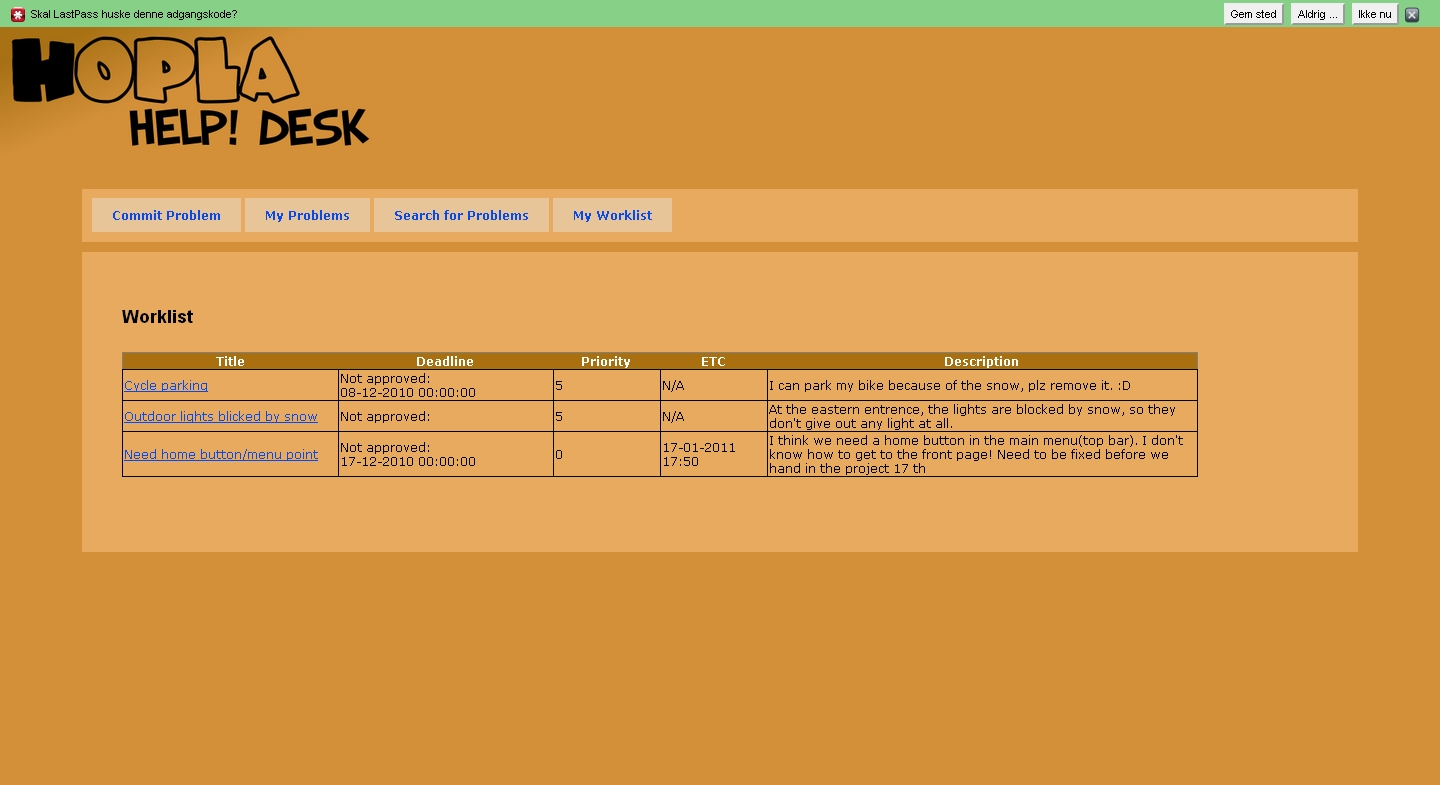
\includegraphics[width=1.00\textwidth, clip=true, trim=4cm 10.5cm 8cm 9cm]{input/magnus_before.png}
	\label{fig:magnus_before}
\end{figure}
\end{frame}

\begin{frame}{Solve Problem}
\begin{figure}[H]
	\centering
		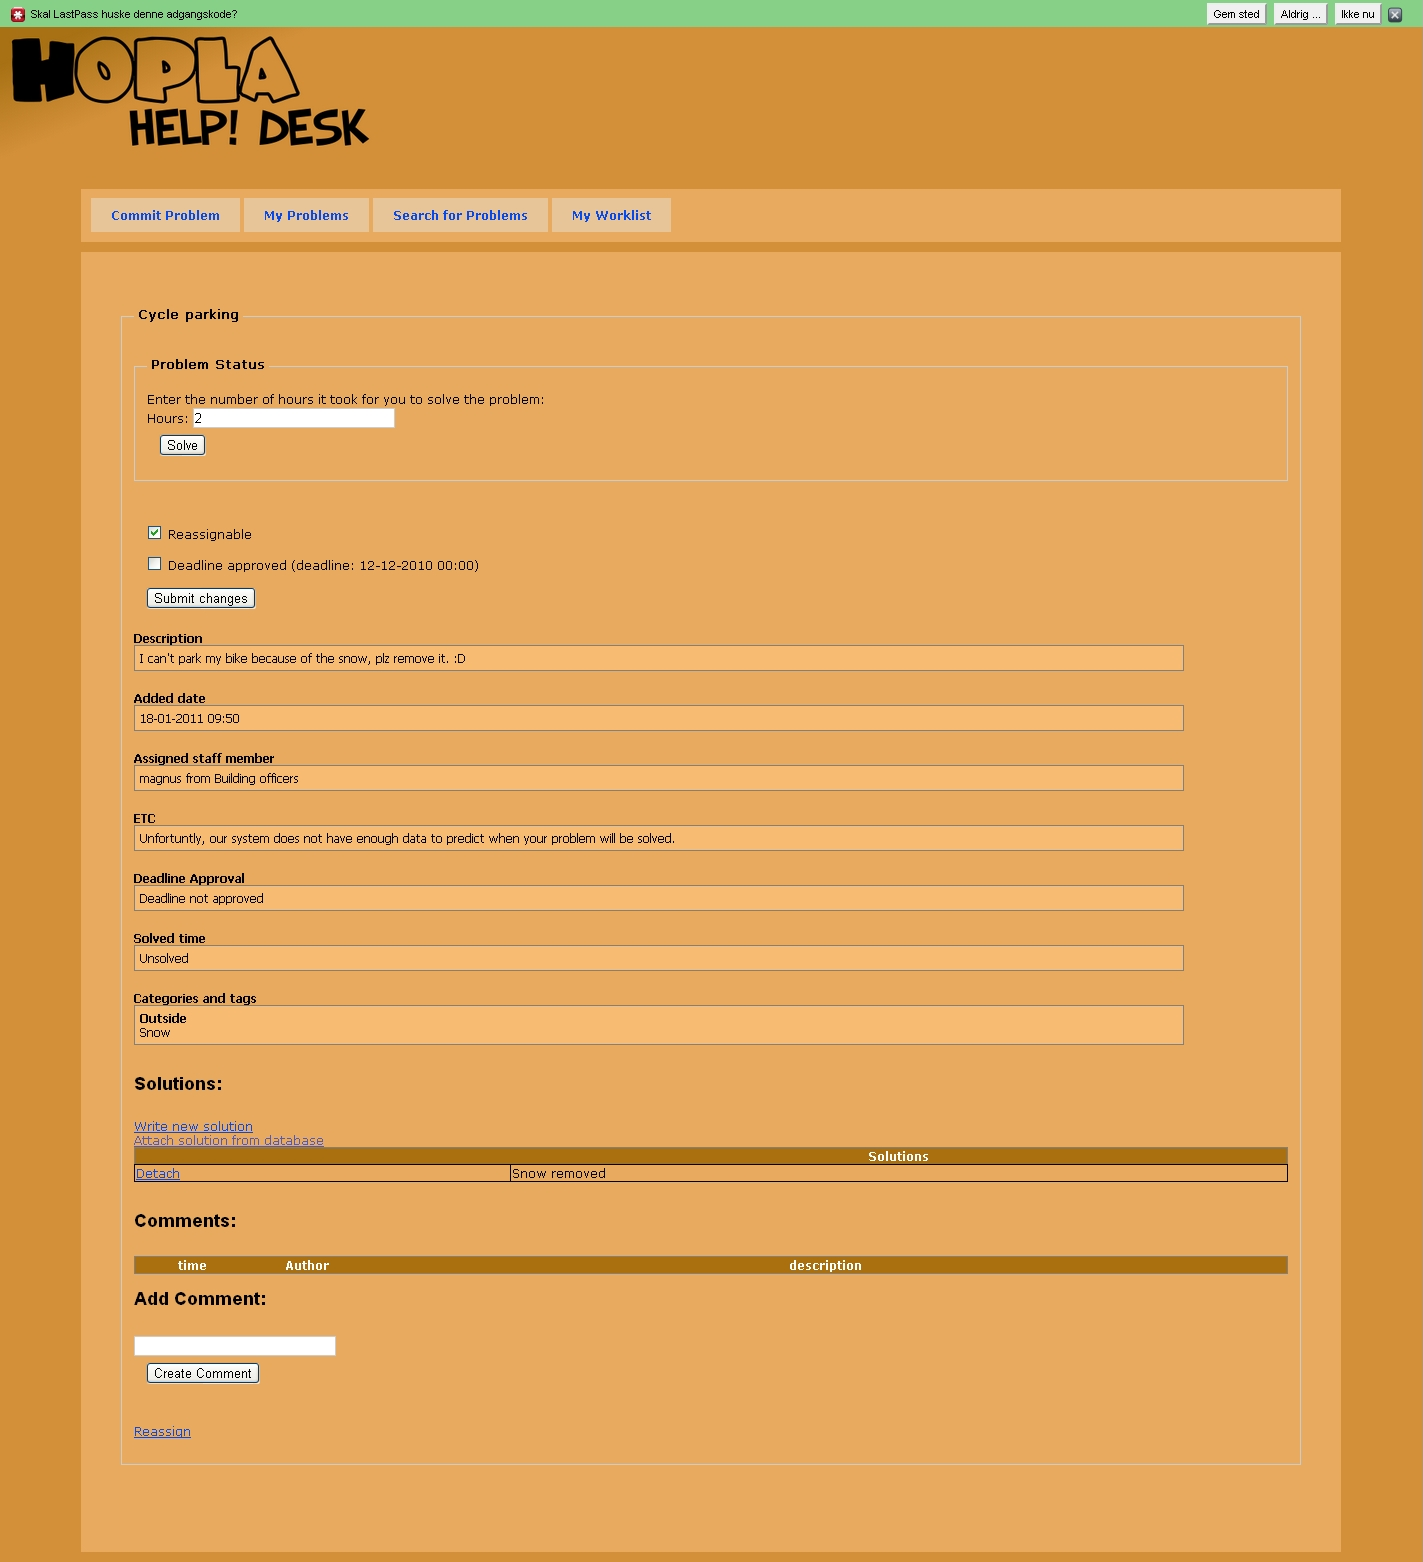
\includegraphics[width=0.90\textwidth, clip=true, trim=4cm 12.5cm 8cm 9.5cm]{input/magnus_solve.png}
	\label{fig:magnus_solve}
\end{figure}
\end{frame}

\begin{frame}{Solve Problem}
\begin{figure}[H]
	\centering
		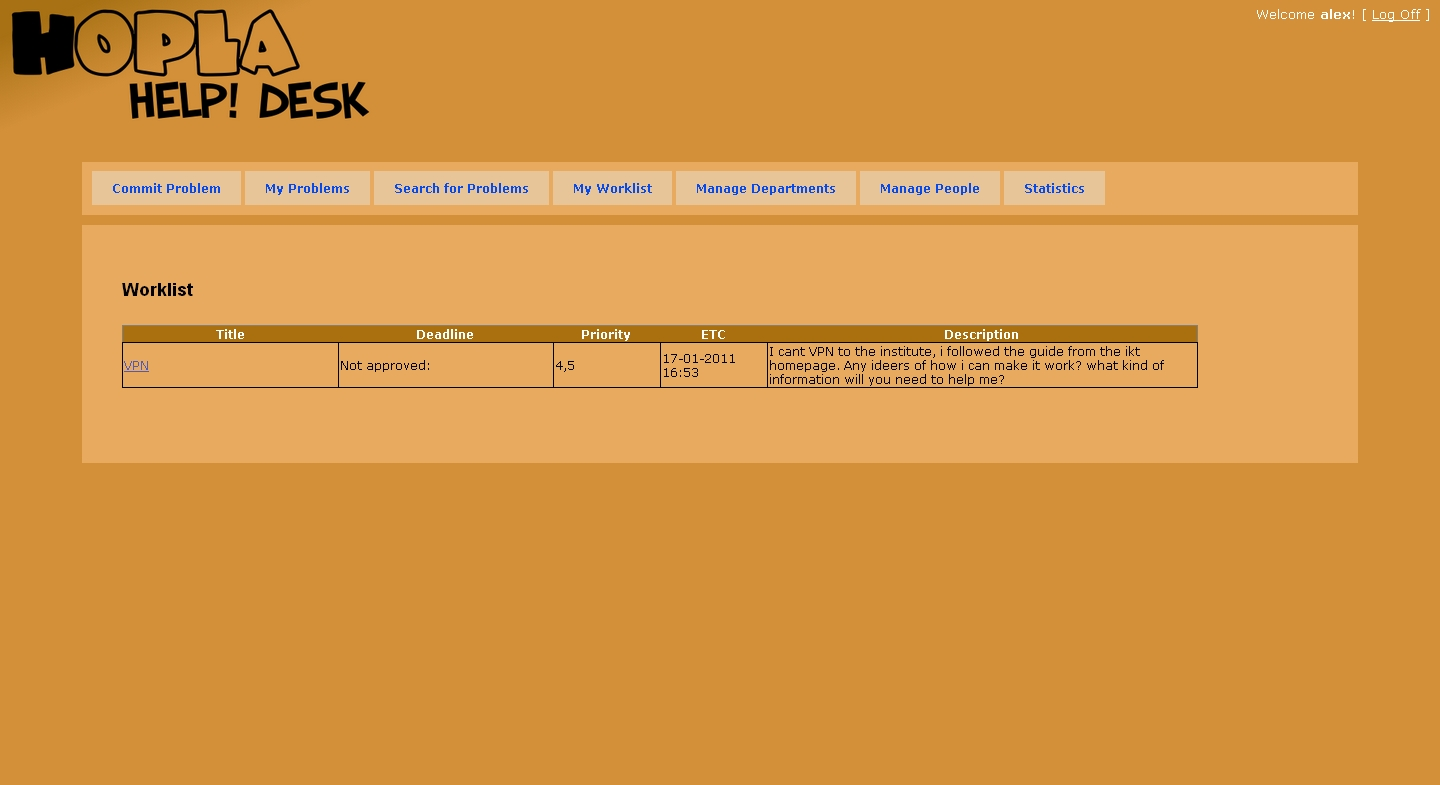
\includegraphics[width=1.00\textwidth, clip=true, trim=4cm 11.5cm 8cm 8cm]{input/alex_after.png}
	\label{fig:alex_after}
\end{figure}

\begin{figure}[H]
	\centering
		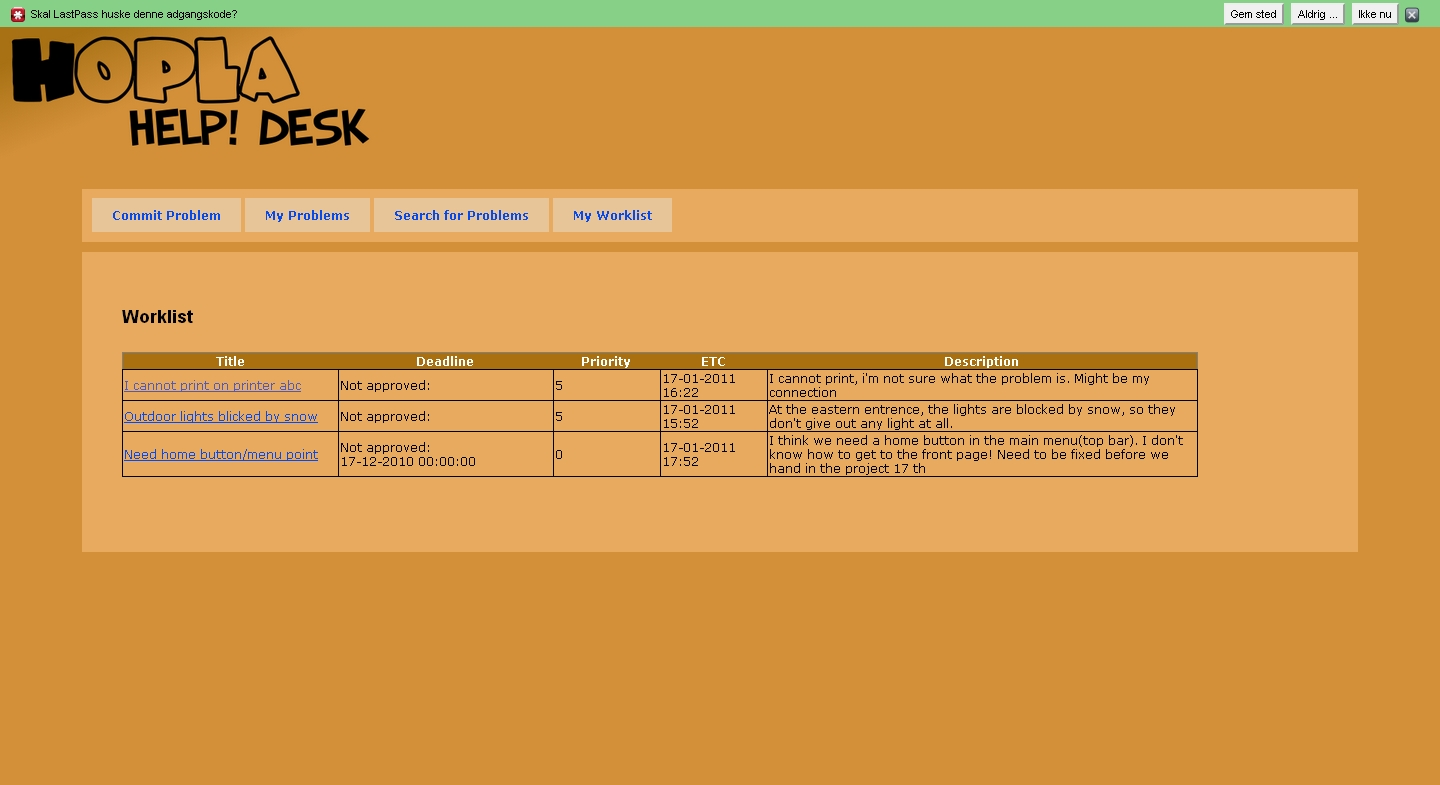
\includegraphics[width=1.00\textwidth, clip=true, trim=4cm 10.5cm 8cm 9cm]{input/magnus_after.png}
	\label{fig:magnus_after}
\end{figure}
\end{frame}

\subsubsection*{Balance Workload}
\begin{frame}{Balance Workload}
\only<1>{
\begin{itemize}
	\item Iterating $n-1$ times
	\begin{itemize}
		\item $n$ is the number employees in department
	\end{itemize}
	\item Balance between maximum and minimum workload
\end{itemize}
}
\only<2>{
\begin{figure}
	\centering
		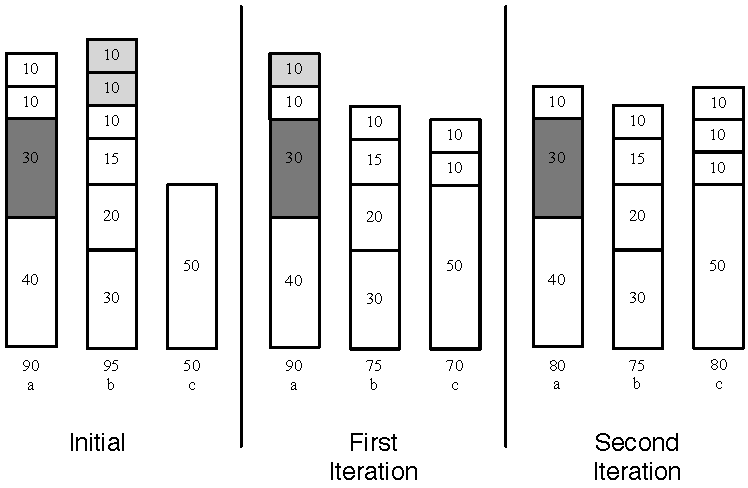
\includegraphics[scale=0.5]{input/balanceWorkloadDiagram.pdf}
	\caption{Found on page 80}
	\label{fig:balanceWorkloadDiagram}
\end{figure}
}
\end{frame}

\begin{frame}{Balance Workload -- Improvements}

\begin{itemize}
	\item Consider priority

	\begin{enumerate}
		\item<2-> Put all reassignable, unsolved problems into a list
		\item<3-> Sort the list
		\item<4-> Assign must important problem to least occupied person
		\item<5-> Repeat step 3 until all problems are assigned
	\end{enumerate}

\end{itemize}

\end{frame}